%Exp 1-9
 \chapter{Waves I: Standing Waves}
\label{chap:waves}
\section{Introduction}
Waves exist in many forms commonly encountered in daily life. For example, your radio receives signals by means of electromagnetic waves and emits sound waves that are measurable by our ears. Waves can exist in many forms including electromagnetic radiation (such as visible light), sound waves, or even vibrations through solid materials (such as waves that exist in bodies of water). Even the human body creates waves (like heartbeats) and diagnostics of the body's physical condition involve many different kinds of wave phenomena. The natural and technological worlds have many examples of waves and understanding their behavior is important in understanding many aspects of the physical world. \myskip

All waves share certain mathematical similarities. In this experiment, we will gain experience with the most important properties of waves\footnote{A general discussion of waves is treated in Chapter 16 of \emph{Fundamentals of Physics} by Halliday, Resnick \& Walker. See Section 16-13 for standing waves. Electromagnetic Waves are covered in lecture next semester. This experiment should familiarize you with the phenomenology of waves.}.

\section{Theory}
\subsection{Waves}
Waves are mathematical objects that depend on a spatial coordinate $x$ and time $t$ in a period manner (such as $\sin$ or $\cos$). In this lab, we will illustrate properties of waves by examining standing waves in a stretched string and sound waves in an air column. \myskip

To be able to describe waves, we introduce a number of definitions:
\begin{itemize}
\item One complete cycle occurs when the mathematical description of a waves repeats itself.
\item The period $T$ is the time it takes for a wave to complete a single cycle.
\item The frequency $f$ , defined as $f = 1/T$, measures the number of complete cycles the wave repeats in one second. The unit of frequency (1/seconds) is Hertz (Hz).
\item The wavelength $\lambda$ is the \underline{spatial} separation between repeating points in a wave.
\item The amplitude $A$ of the wave is the maximum magnitude of the wave.
\end{itemize}

If a long, taut horizontal string is sharply pulled up at some point and released, this part of the string will vibrate up and down. Neighboring points will then follow the motion, and the original disturbance will propagate down the string as a ��traveling wave��. Since the individual particles vibrate in a direction perpendicular to the direction of propagation, this wave is called a transverse wave. If the disturbance is periodic, i.e., repeated continuously, a wave train will move down the string. The following figure shows the disturbance along the string at a single instant of time, in this case for a sinusoidal wave. If the wave is moving to the right and a second picture is taken a quarter period, $T/4$, later, all points on the wave will have moved an equal distance to the right, as shown by the dotted curve. The frequency, $f$, of the wave is defined as the number of times per second the disturbance is repeated (thus $f = 1 / T$). Note that the period of the motion is determined by the cause of the initializing disturbance. During each period $T$, the wave travels a distance of one wavelength, $\lambda$; therefore the velocity of the wave is given by\footnote{In all the cases here, $c$ will be a constant. But in general $c$ could be a function of the frequency. (This effect is called dispersion).} $c=f\lambda$.\myskip
\begin{figure}[h]
\centering
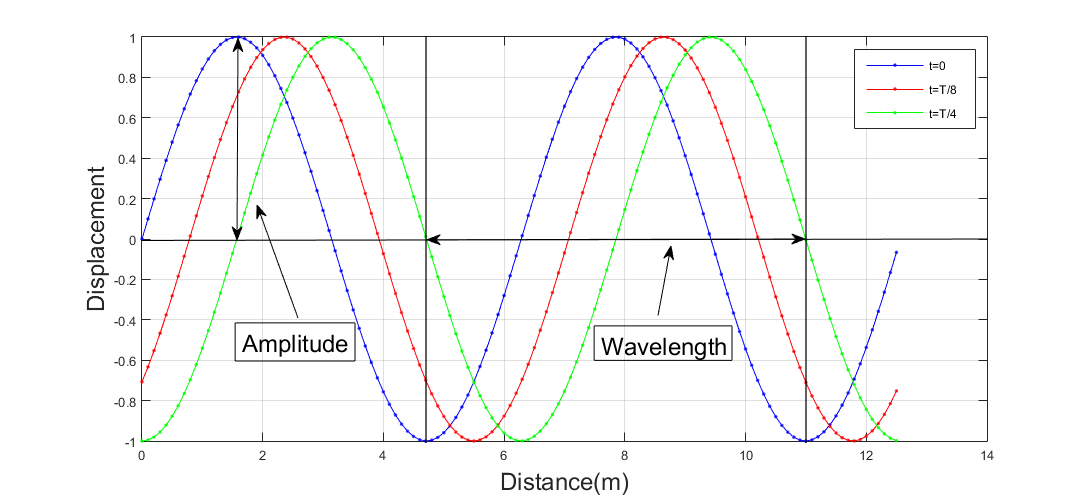
\includegraphics[width=1.0\textwidth]{./Exp1-9/pic/page01.png}
\caption{Propagation of a transverse traveling wave at 3 different times: $t=0$, $t=\tau/8$, and $t=\tau/4$}
\end{figure}


The figure below shows the vertical displacement of the string versus time at a fixed location along the string. The time interval between successive identical displacements of a given point is the period $T$ of the wave. Remember that the wavelength of a traveling wave can only be determined when one observes the displacement as a function of distance at one instant in time. The period, on the other hand, is obtained when one observes the displacement of one point as a function of time at one location.\myskip
\begin{figure}[h]
\centering
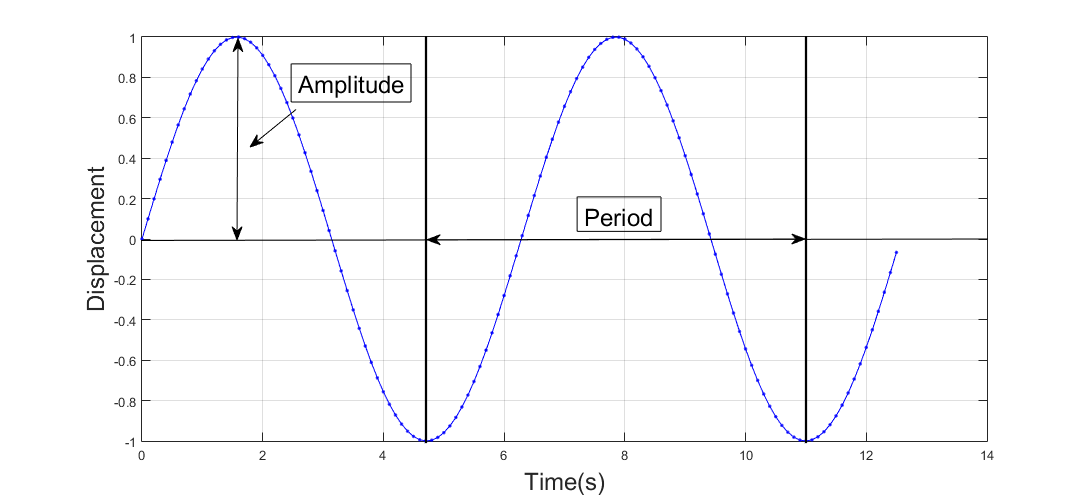
\includegraphics[width=1.0\textwidth]{./Exp1-9/pic/page02.png}
\caption{Vertical displacement of a vibrating string as a function of time}
\end{figure}

There are, in general, two types of waves: transverse and longitudinal. If the oscillation is perpendicular to the direction of propagation of the wave, then the wave is transverse\footnote{The two independent possibilities for making a transverse wave are referred to as the two possible polarizations of the wave. (If the wave oscillates diagonally, it can be viewed as a combination of vertical and horizontal polarizations.)}. If a wave changes \underline{along} the direction of propagation, it is called a longitudinal wave. \myskip

An example of a longitudinal wave is a sound wave, in which there are periodically changing regions of low and high air pressure along the direction of wave propagation. A sound wave is normally initiated by a vibrating solid (such as a tuning fork), which alternately compresses and rarefies the air adjacent to it. The wave thus consists of pressure variations in the air that are moving away from the fork. Since these variations oscillate along the direction of wave propagation, the sound wave is a longitudinal traveling wave.\myskip

The definitions of $f$, $\lambda$ , and $T$, explained above for transverse waves, hold equally for longitudinal waves. The diagrams in the above figures also apply, so long as we understand ``displacement'' to mean the longitudinal (forward or backward) pressure or density variation of air from its undisturbed equilibrium value. The relationship between wave velocity and the other parameters is also still valid:
\begin{equation}
  c=f\lambda
\end{equation}

\subsection{Standing Waves}

So far we have considered only very simple wave disturbances. More complicated waves are created when two or more traveling disturbances are present simultaneously in the same medium. There is a law of superposition which states that the position of a given point on the medium is determined by the sum of all the different disturbance effects. In general, any number of waves can be combined to give a more complicated wave.\myskip

A particularly interesting example occurs when two waves of equal $\lambda$, $f$, and $A$ are traveling along a taut string in opposite directions. (This occurs if the wave encounters a barrier that reflects the wave back in the original direction while the original wave is still propagating.) At some particular points on the string, the two waves will always be out of phase, one wave will try to move the point up and other wave will try to move the point down. The result is that the two waves will cancel each other at this particular point, and so that point will remain stationary. This condition is known as destructive interference, and the points at which this occurs are called nodes. \myskip

At other points on the string, the two waves will move up and down together so that the amplitude of the disturbance at these points will be twice what it would be if only one wave were present. This condition is known as constructive interference and the points at which this occurs are called antinodes. \myskip

As long as the $\lambda$, $f$, and $A$ of the waves remain fixed, the positions of the nodes and antinodes will not change. The pattern produced in this circumstance is called a standing wave, since it looks as if it is stationary, although it is actually the sum of two waves traveling in opposite directions. The analytic description for the displacement $\Psi$ versus position and time with one end fixed at $x$ = 0 is given by:
\begin{equation}
\Psi (x,t) =  A\sin\bigg(\frac{2\pi}{\lambda}x\bigg)\cos\bigg(2\pi f t\bigg)
\end{equation}

A string with both ends fixed can be excited with standing waves as shown in the figure below. The fixed ends of the string cannot move, so the string must have nodes at these points. It is evident that the distance between the node at a fixed end and the first antinode is $\lambda /4$; and the distance between successive nodes (or antinodes) is $\lambda /2$.\myskip
\begin{figure}[h]
\centering
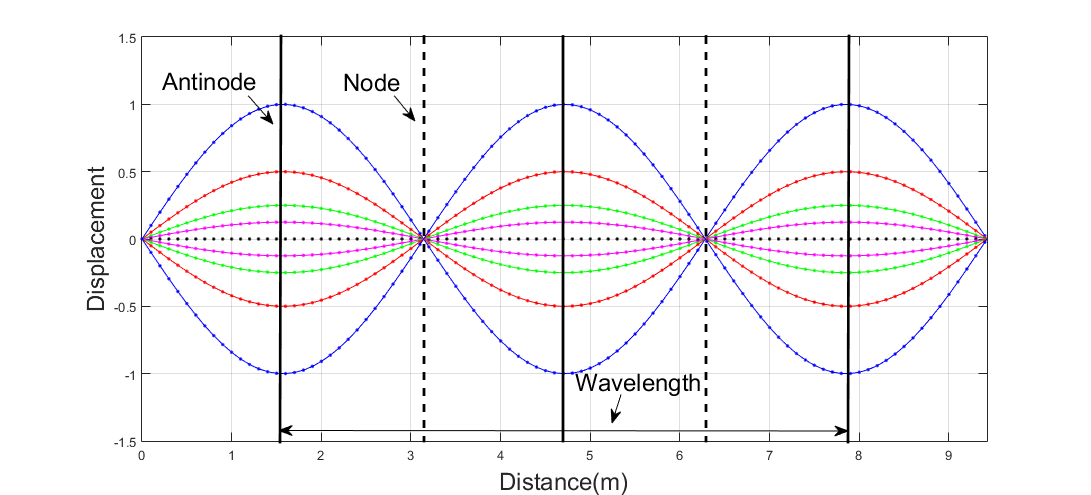
\includegraphics[width=1.0\textwidth]{./Exp1-9/pic/page04.png}
\caption{Standing waves at various times. The nodes and anti-nodes reside at fixed distances. The amplitude of the oscillations oscillate in time according to equation (8.2)}
\end{figure}

 The positions on the string where $A\sin(2\pi x/\lambda) = 0$ correspond to a node, so whenever $2\pi x/\lambda$ is a multiple of $\pi$, i.e.:
 \begin{equation}
   \frac{2\pi}{\lambda}x=n\pi
 \end{equation}
($x$ is a multiple of $\lambda$/2), we find a node. Midway between two nodes we will always find an antinode, a point where the string oscillates maximally.

Standing waves can be created in a tube of gas using sound waves. In this part of the experiment, a tuning fork vibrates over the open end of a tube containing air. The tube is sealed at the other end by the water. The motion of the fork causes longitudinal sound waves to travel down the tube. The sound wave is reflected back up by the air-water interface and the incident and reflected waves interfere with each other. The air at the closed end of the tube is cannot move freely, so in order for a standing wave to be produced, a node must exist at the there. The air in the open end of the tube is free to move; so when a standing wave is produced in the tube, the open end is an antinode.\myskip

Since the distance between a node and the nearest antinode in a standing wave pattern is $\lambda/4$, it should be evident that the shortest tube in which a standing wave can be established has a length of $\lambda/4$. A standing wave with wavelength $\lambda$ can be established in longer tubes. All that is required is that a node exist at the closed end and an antinode at the open end -- i.e. that the length of the air column is an odd multiple of $\lambda/4$. When a standing wave is produced in the tube, a resonance condition is established and the intensity of the sound will increase.

\section{Experiments}
\subsection{Standing waves on a String}
The first part of the experiment deals with transverse waves on a string. A long horizontal string is attached to the tine of a driven tuning fork that vibrates at $f = 60\, \textrm{Hz}$. The other end is fixed at a point where it passes over a pulley. You can change the distance between the pulley and the tuning fork by shifting the base of the tuning fork and you can hang weights of mass $M$ on the end of the string (which produces a string tension $T=Mg$). The apparatus is pictured in the figure below:\myskip
\begin{figure}[h]
\centering
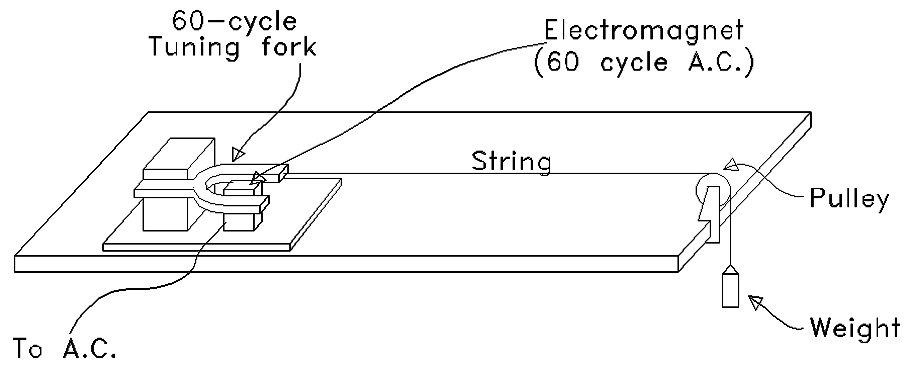
\includegraphics[width=0.8\textwidth]{./Exp1-9/pic/image4.png}
\caption{Experimental setup for measuring the wavelengths of standing waves}
\end{figure}

Your task is to measure the wavelengths resulting from standing waves produced for various values of the tension. In the previous section, it was stated that the distance between two nodes in a standing wave is $\lambda/2$. So the wavelength is double the distance between adjacent nodes.\myskip

Measure the mass and length of the string. Calculate $\mu$, the linear density of the string. Attach the string to the screw on the tuning fork and place it over the pulley. Put a mass of $100\, \textrm{g}$ on the end of the string and choose the distance between pulley and tuning fork such that you get a standing pattern of nodes and anti-nodes.
\begin{enumerate}
\item Measure the wavelength of the standing waves. You get the best results if you measure nodes in the middle of the string and if you average over several measurements.
\item Calculate the velocity with which the wave propagates on the string, using the relation between frequency and wavelength. Include error in measured velocity by propagating uncertainty in wavelength $\lambda$.
\item Analytically calculate the velocity of propagation of waves on a string from the physical properties of the string and equation (9.4). Include error in calculated velocity by propagating uncertainties in tension $T$ and mass per unit length $\mu$.
  \begin{equation}
    c=\sqrt{\frac{T}{\mu}}
  \end{equation}

\item Do your theoretical velocities agree with your experimental values within error?
\item Repeat the series of measurements and calculations for 3 different weights.
\item Discuss the main sources of error in measuring the wave velocity?

\end{enumerate}

\subsection{Standing Sound Waves}

In the second part, we measure the wavelength of standing longitudinal waves.
\begin{figure}[h]
\centering
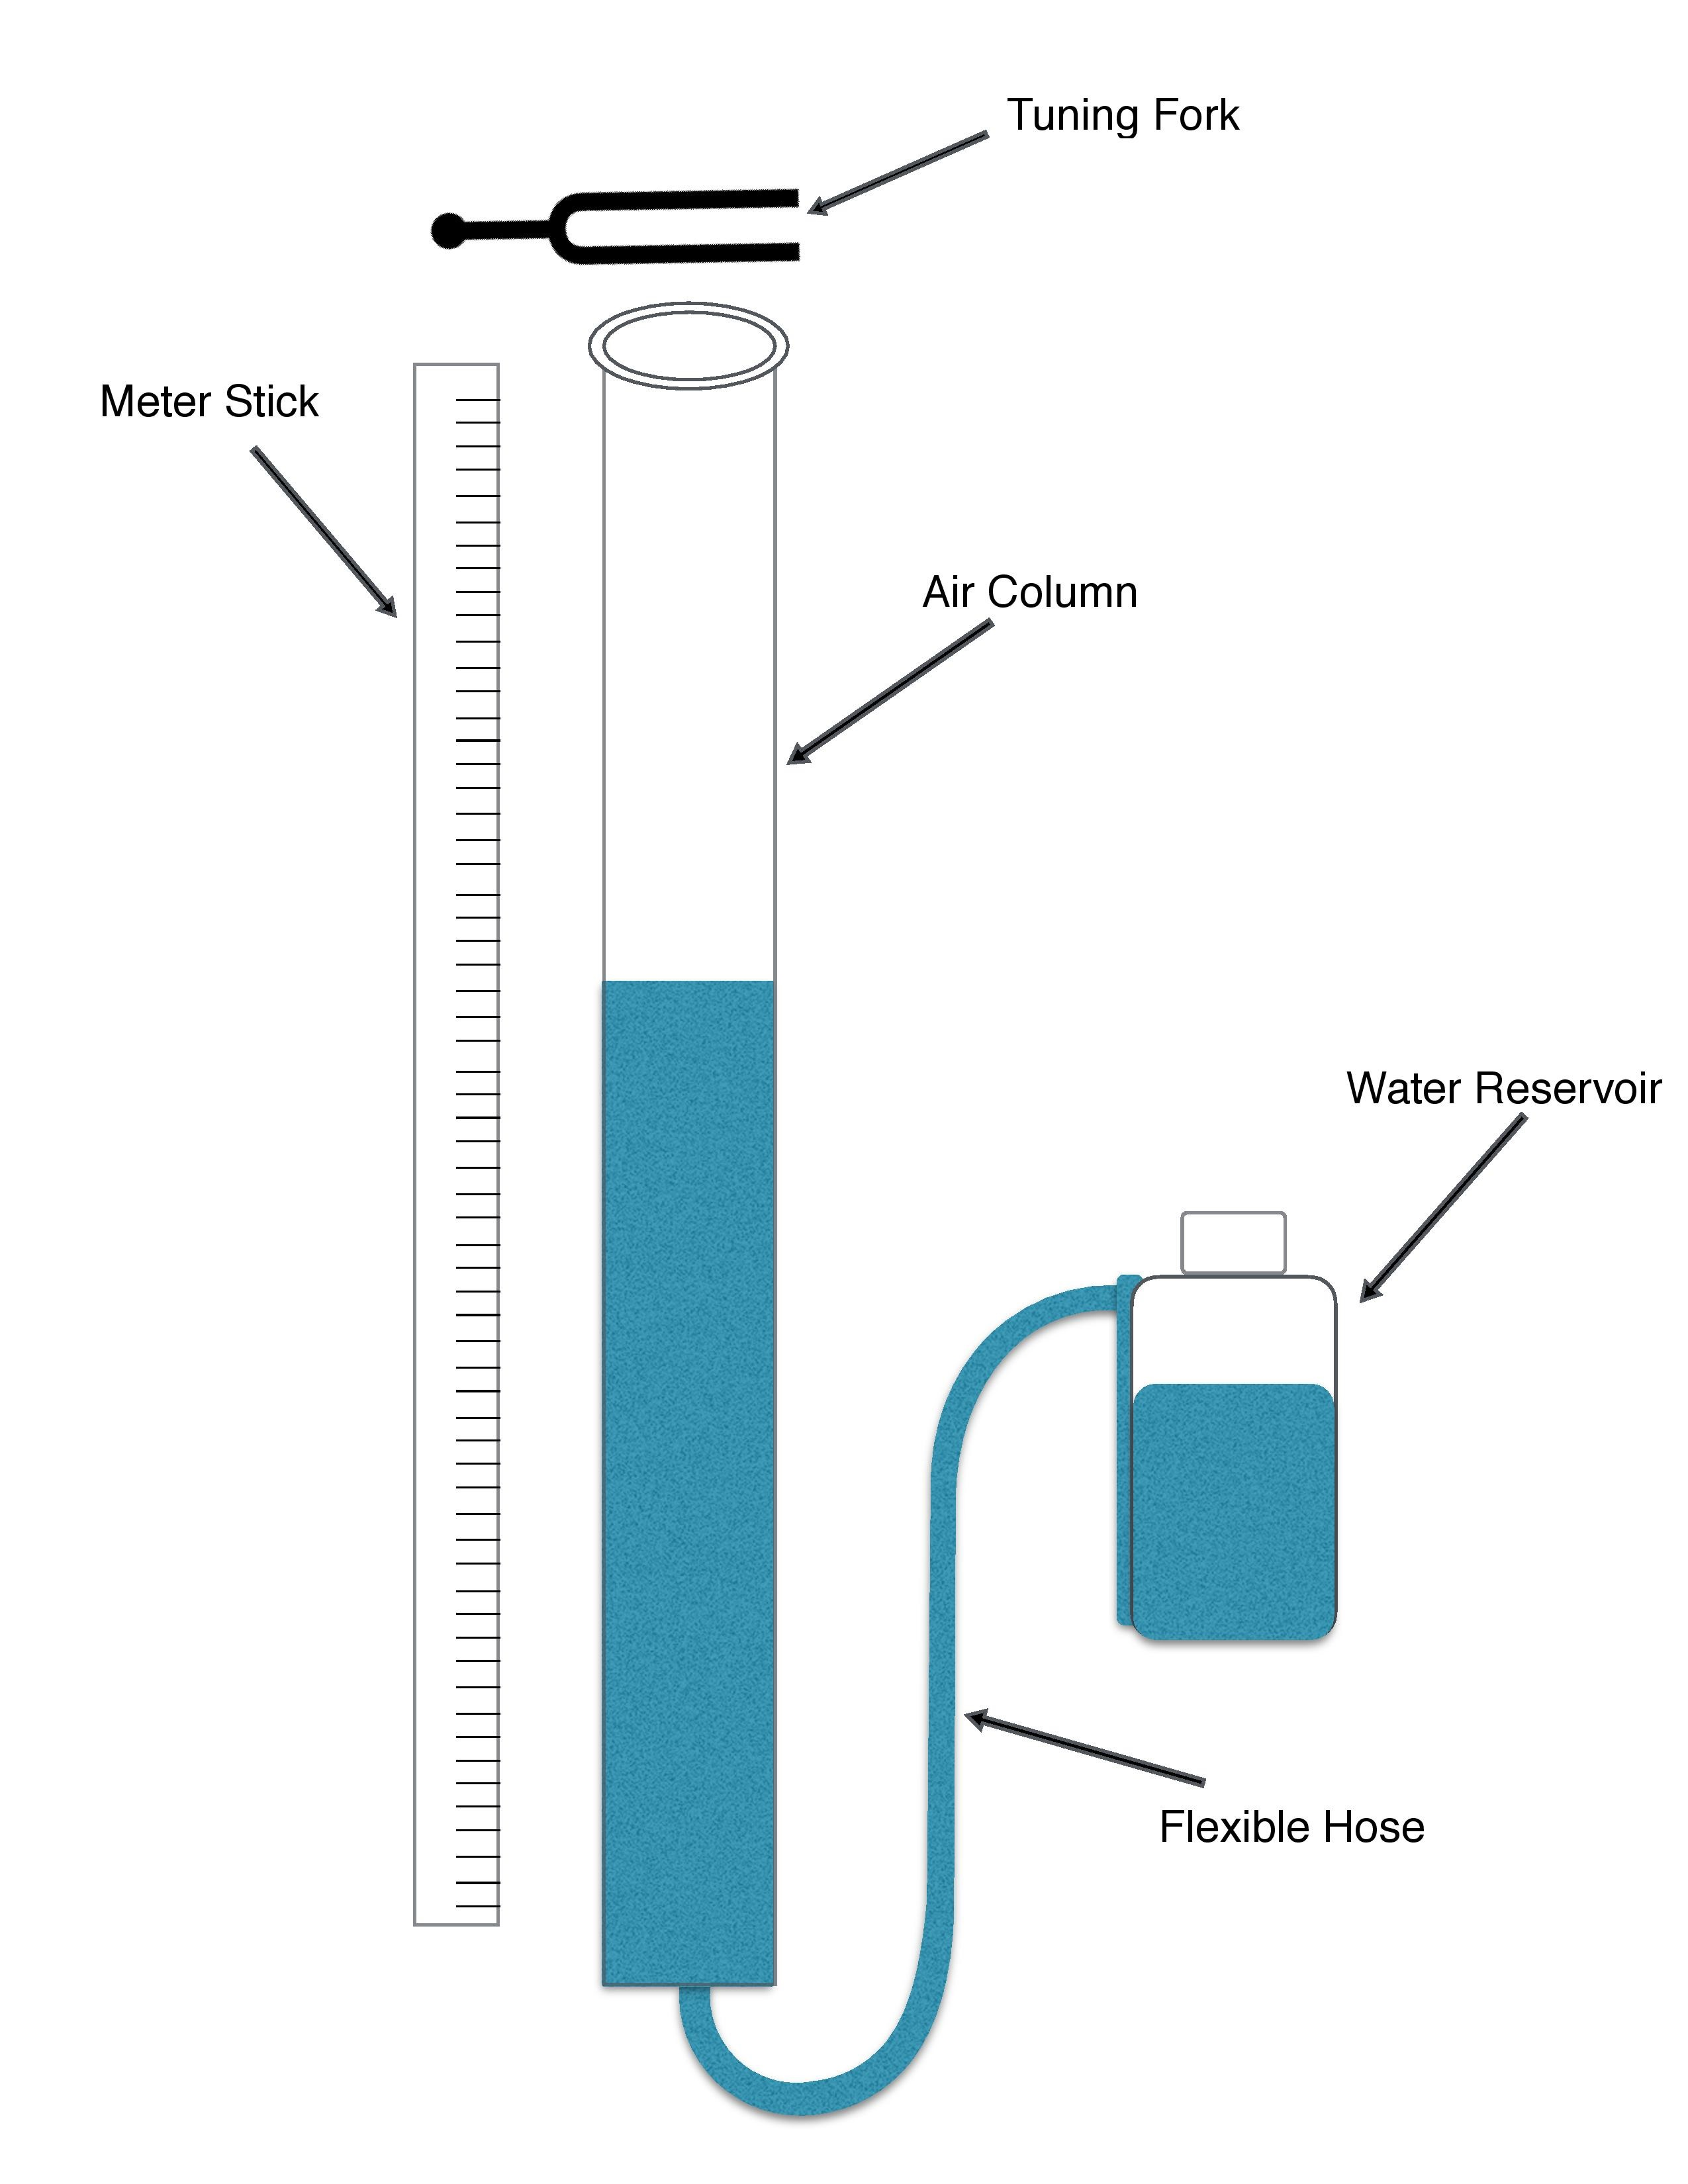
\includegraphics[width=0.7\textwidth]{./Exp1-9/pic/page03.jpg}
\caption{Experimental setup for measuring the wavelengths of standing longitudinal sound waves}
\end{figure}

Sound waves (longitudinal waves) are set up in a long open tube, which is partly filled with water, as shown in the figure to the right. We change the height of the water column by lifting or lowering a water reservoir. Produce a sound wave using a tuning fork. There are two tuning forks, a $512\, \textrm{Hz}$ one and a $1024\, \textrm{Hz}$ one. You should perform the experiment with both of them. Strike the tuning fork and hold it at the top of the glass tube. As you change the level of water in the tube, you find some water levels at which the sound from the tuning fork becomes significantly louder. This occurs whenever you have created a standing sound wave in the glass tube. By measuring the distances between water levels that achieve successive sound maxima, you can determine the wavelengths of the sound waves. \myskip

As before, from the wavelengths of the standing waves and the frequencies, you can compute the velocity of propagation of the sound waves for each case. This should equal the speed of sound in air.\myskip

\underline{\emph{Remark}:} It is often easiest if you lower the water level continuously and hit the tuning fork somewhat hard. However, please be careful and don't damage any equipment.
\begin{enumerate}
\item Measure the wavelength for both tuning forks. There should be small string-rings on the glass tube that you can use to mark the levels at which you get resonance (standing waves). To improve your data try to average over several measured values. Also don't forget to include uncertainties.
\item Calculate the speed of sound for both frequencies. Do you get the same value within uncertainty? Is your value for the speed of sound close to the standard value of $340\,\textrm{m/s}$? What sources of error could contribute to an incorrect calculation for the velocity of sound in air?
%\item Was one of the tuning forks easier to hear than the other? If yes, do you have an idea why?
\item The speed of sound in air is in fact dependent upon the temperature in the room through the following relation:
\begin{gather}
v_\text{sound in gas} = \sqrt{\frac{\gamma R T}{M}}
\end{gather}
Where $\gamma$ is a constant dependent upon the gas (for air $\gamma=1.4$), $R$ is the gas constant ($R=8.31 \frac{\text{J}}{{K} \cdot \text{mol}}$), $M$ is the molar mass of the gas molecules (you may use $M = .029 \frac{\text{Kg}}{\text{mol}}$ for dry air), and $T$ is the temperature of the room in kelvin. Consider the molecules the air to determine which molecular masses to use. Calculate the temperature of the room using this equation for the velocities measured for both  tuning forks. Include error in room temperature by propagating uncertainty in measured velocity $v$.
\item Discuss the main sources or error that might contribute to the calculation of wave velocity.
\end{enumerate}

\section{Applications}
Biological systems that create periodic pulses (like a beating heart) are optimized for a range of operating conditions. The variations in the operating parameters often provide an important diagnostic tool. For example, the period of beats in a human heart can vary; one may ask to what extent and how often the heartbeat rate changes. To identify patterns of heart rate, one makes use of a mathematical procedure called Fourier analysis. Besides the dominant frequency of the heartbeat (about $1\, \textrm{Hz}$), there are other frequencies that correspond to changes in the heart rate; Fourier analysis uses the heart rate to make a diagram of the amplitudes of the lower frequencies present in the heart rate. \myskip

This may at first sound a little bit complicated, but the basic idea is simple. In the experiment, we find only specific standing waves for each system. With the system parameters fixed, only certain frequencies are possible: most frequencies cannot achieve a standing wave. Obviously these frequencies are special and characterize the system! If you look now at a complicated oscillation of the system and take the Fourier spectrum, you find that only these special frequencies contribute. Other frequencies don't contribute at all. A beating human heart is, of course, much more complicated than the systems we deal with in the lab, but the basic ideas are the same!\myskip
\begin{figure}[h]
\centering
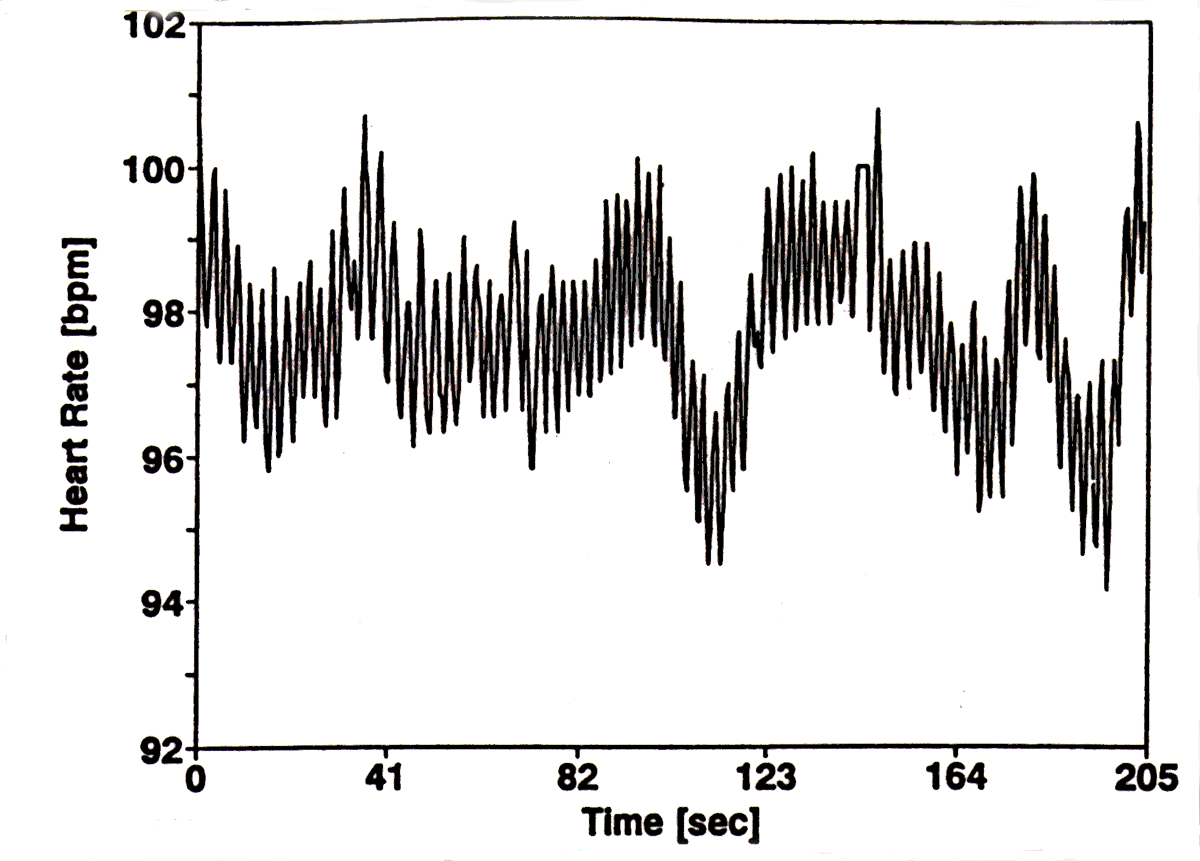
\includegraphics[width=0.8\textwidth]{./Exp1-9/pic/image6.png}
\caption{Heart rate of an adult as a function of time}
\label{fig:heart}
\end{figure}

This picture shows the heart rate of a healthy adult over time. As one can easily see, the heart rate changes over time. The frequencies with which the heart rate changes can most easily be seen in the Fourier spectrum (sometimes called power spectrum) in the next figure.\myskip
\begin{figure}[h]
\centering
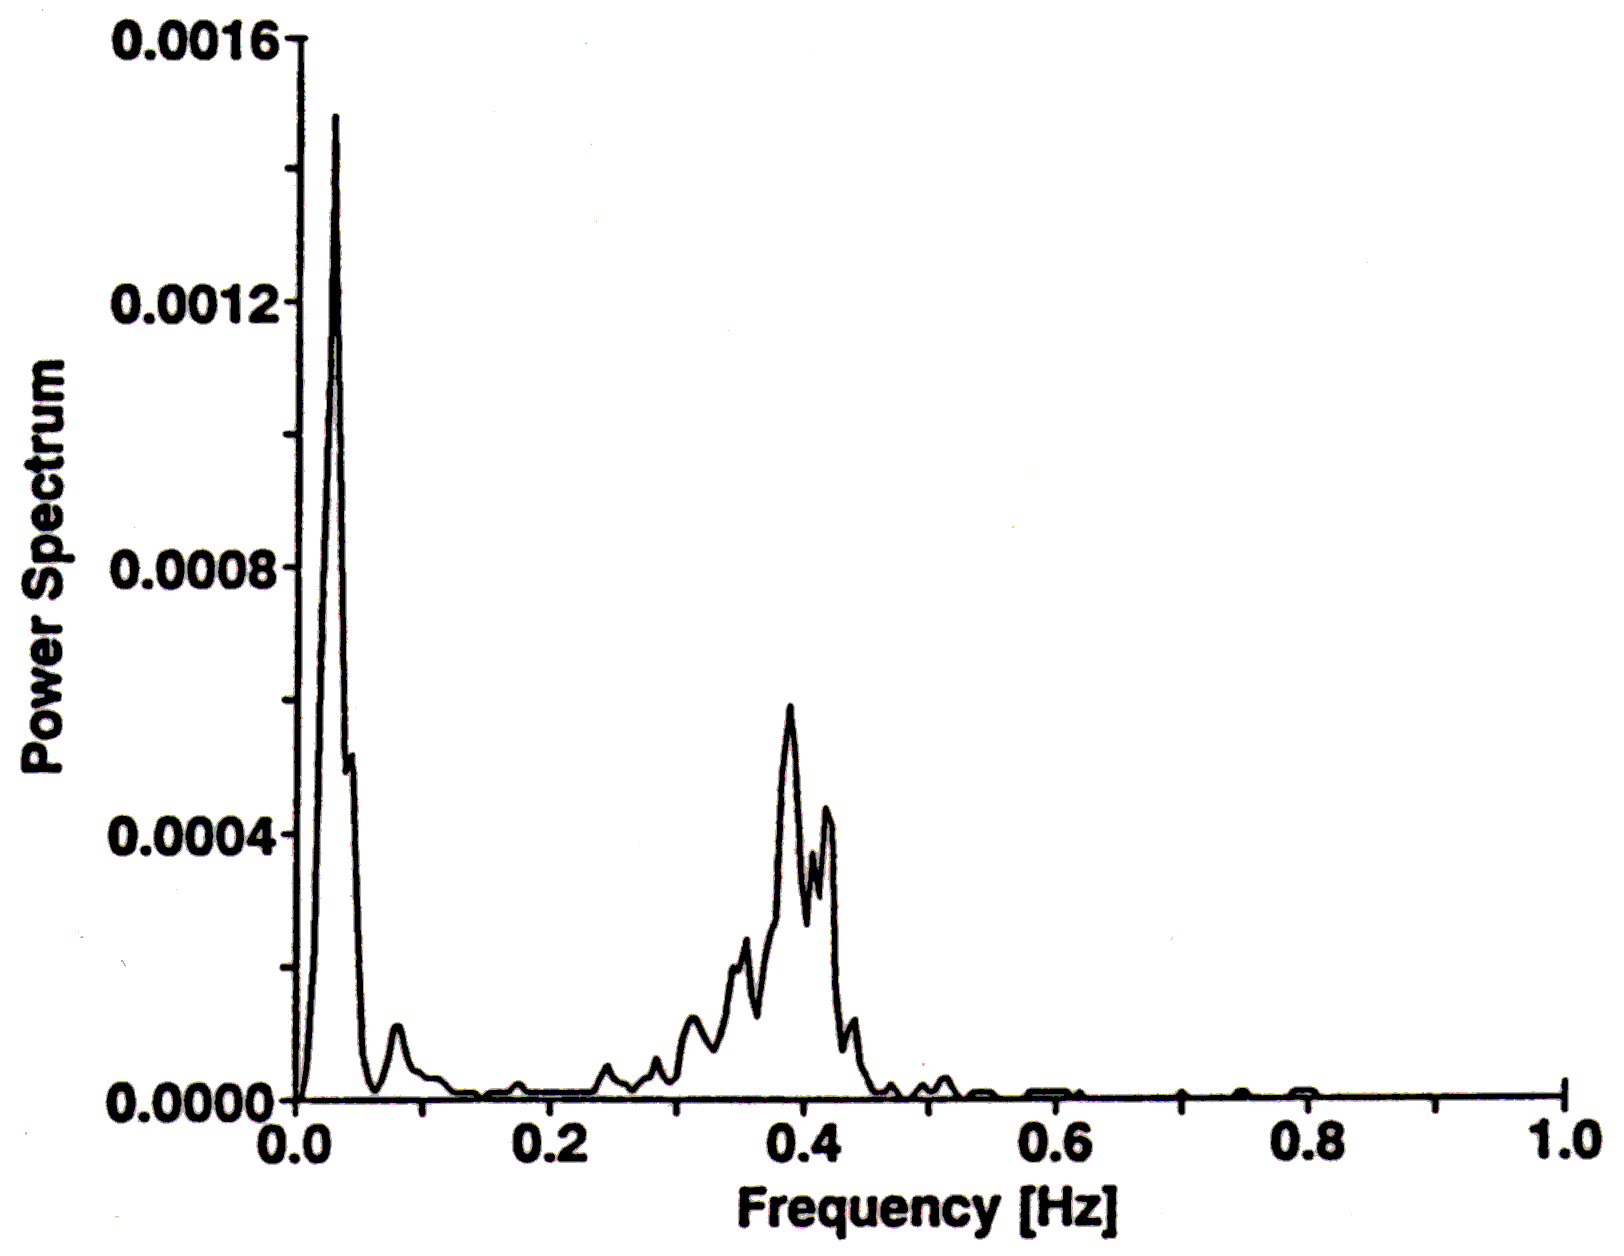
\includegraphics[width=0.8\textwidth]{./Exp1-9/pic/image7.png}
\caption{Power spectrum of the adult heart rate plotted in figure \ref{fig:heart}}
\end{figure}

One immediately sees a prominent change in the heart rate with a frequency of about $0.4\, \textrm{Hz}$. Therefore, roughly every $2.5\, \textrm{s}$ the heart rate of this person changes. This frequency corresponds to the many little spikes we saw in the first diagram. (Another characteristic frequency is at about $0.02\, \textrm{Hz}$, corresponding to a change about every $50\, \textrm{s}$. We will not deal with this part here, even though it contains valuable information.)\myskip

Where does the change every $2.5\, \textrm{s}$ come from? It turns out that the person took a breath about every $2.5\, \textrm{s}$. The heart then speeds up slightly to pump more blood through the vessels of the lung, where the blood is oxygenated. Subsequently, it slows down again. (This particular frequency is called the respiratory frequency.)\myskip

The process of speeding up and slowing down is governed by the autonomic nervous system. Some diseases (e.g. diabetes) can damage the autonomic nervous system and therefore stop this adaptation of the heart rate. For example, as diabetes reaches its final stage the peak in the Fourier spectrum at the respiratory frequency vanishes. \myskip

This method has the nice feature that it is non-invasive, relatively simple, and shows dynamic processes rather than snapshot pictures.\myskip

\emph{Reference:} Amos D. Korczyn: Handbook of Autonomic Nervous System Dysfunction.
\section{Lab Preparation Problems}
\myskip
{\bf{Note: Suggested prelab questions are in bold. These will help will conceptual understanding of the laboratory experiments.}}
\\
\\
\noindent\underline{Waves}:\myskip

{\bf{1. Is a wave on the water surface a longitudinal or transverse wave?}}\myskip

2. The wavelength of visible light is between $400$-$800\, \textrm{nm}$. What is the frequency of visible light?\myskip

\noindent\underline{Standing Waves}:\myskip

 3. A transformer is humming at a frequency of $60\, \textrm{Hz}$ and produces a standing wave in air. What is the distance between adjacent nodes? What is the distance between adjacent antinodes? \myskip

4. You have a string and produce waves on it with $50\, \textrm{Hz}$. The wavelength you measure is $7\, \textrm{cm}$. What is the speed of the wave on this string?\myskip

{\bf{5. You put a mass of $400\, \textrm{g}$ on the string of experiment 1. (The string is $50\, \textrm{cm}$ long and weights $12.5\, \textrm{g}$) What distance between adjacent nodes do you then expect for a frequency of $100\, \textrm{Hz}$. (Use $g = 10\, \textrm{m/s}^2$)}} \myskip

{\bf{6. With a $660\, \textrm{Hz}$ tuning fork you measure a distance of $25 \pm 2\, \textrm{cm}$ between adjacent nodes. Is the value of $c = 340\, \textrm{m/s}$ within the uncertainty of your measured value?}}\myskip

\noindent\underline{Explanations}:\myskip

{\bf{7. If you blow air along the top of an open soda bottle you can excite a standing wave in the bottle and you hear a sound. Explain what happens if you put some water into the bottle and then perform the same experiment!}} \myskip
